\chapter{LHCb Detector}\label{chap:02}

\section{}

\begin{figure}[H]
    \centering
    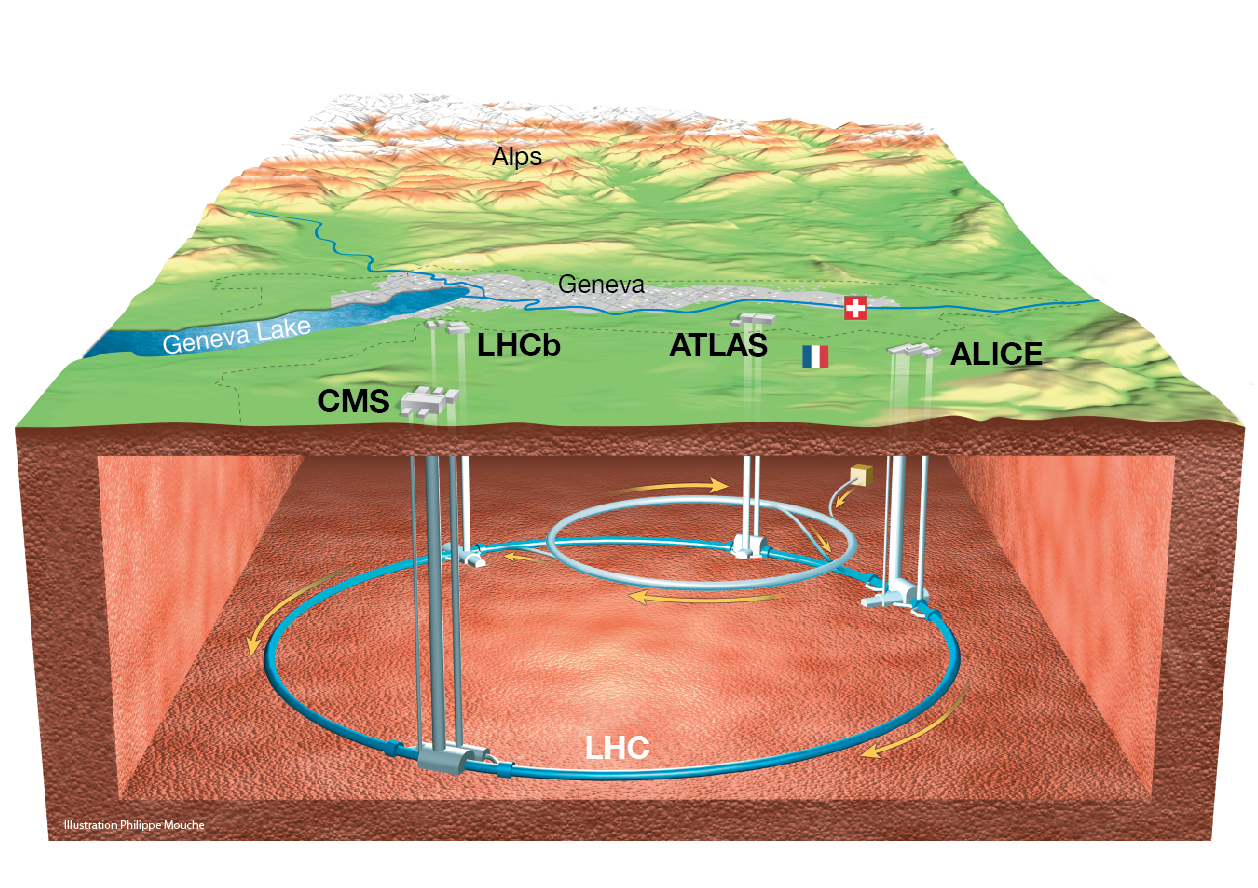
\includegraphics[width=0.7\linewidth]{images/LHC_scheme.png}
    \caption{LHC schema with ALICE, Atlas, CMS and LHCb at CERN.}
    \label{LHC}
\end{figure}

The LHCb detector is part of one of the four large experiments set up on different points of the circular accelerator design of LHC, at CERN. The detectors are constructed around collision points where the accelerated beams of protons are crossed with each other \( 40 \times 10^{16} \) times per second. Unlike rest of the detectors at LHC, the LHCb detector is built to detect particles from a singular direction, with the official name for the design being, "Single arm forward spectrometer". It can detect particles coming from the interaction point in the pseudorapidity range between 2 < η < 5 and it is design philosophy is geared towards measuring b (bottom) and c (charm) hadron properties alongside CP violation. \cite{LHCb_detector}


\begin{figure}[H]
    \centering
    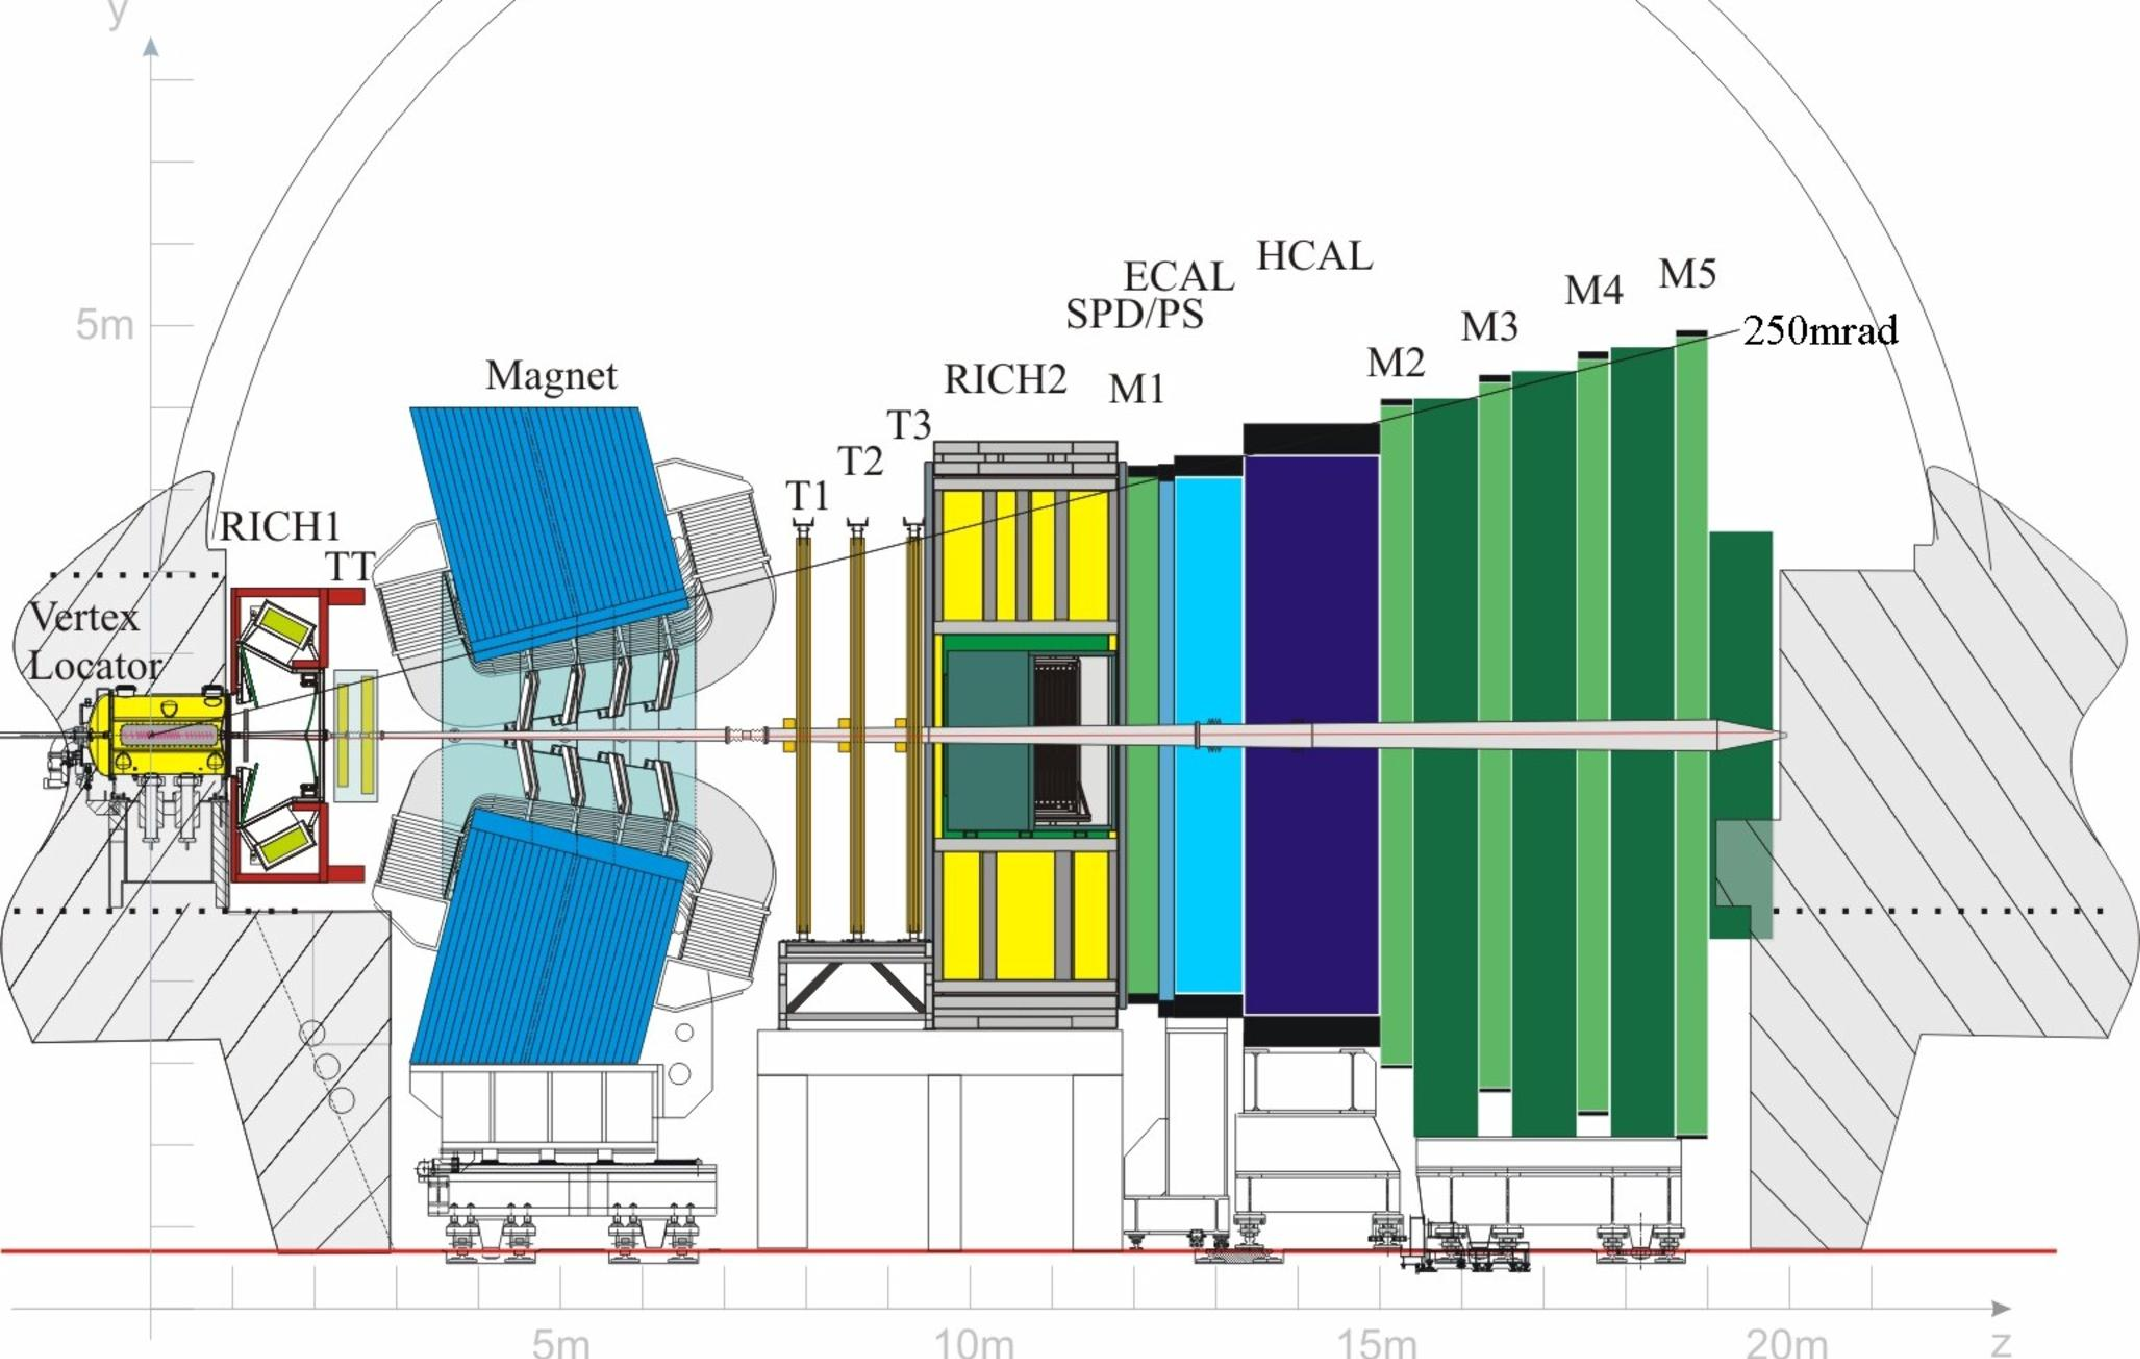
\includegraphics[width=0.7\linewidth]{images/LHCb_diagram.png}
    \caption{The LHCb detector. Detector elements from left to right:  I-Vertex locator, II-Ring imaging Cherenkov detector 1, III-Trigger tracker(TT), IV-Dipole magnet, V-Outer trackers(T1,T2 and T3), VI-Ring imaging Cherenkov detector 2, VII-Muon detector 1, VIII-Hadronic and electromagnetic calorimeters, IX-Muon detector 2,3,4 and 5.}
    \label{LHCb}
\end{figure}

The LHCb detector is made up of the following components:
%--------------%
\begin{enumerate}[label=\textbf{\arabic*.}]
    \item \textbf{VELO (Vertex locator)}
    
    \textbf{Purpose:} Precise reconstruction of primary and secondary vertices coming \\from the collision.
    
    \textbf{Features:} Silicon-strip detectors close to the beam line, retractable during the beam injection phase.
%--------------%
    \item \textbf{TT Station (Trigger tracker)}
    
    \textbf{Purpose:} Tracking particles before entering the magnetic field.
    
    \textbf{Features:} Silicon microstrip detector upstream of the magnet.
%--------------%
    \item \textbf{Dipole magnet}
    
    \textbf{Purpose:} Bends charged particles, making it possible to measure their momentum later.
        
    \textbf{Features:} Approximately 4 T$\cdot$m integrated magnetic field special to the forward spectrometer design.
%--------------%
    \item \textbf{Tracking stations (T1,T2 and T3)}
    
    \textbf{Purpose:} Tracking particles after leaving the magnetic field (tracking charged particles for momentum measurement).
    
    \textbf{Features:} Straw tube drift chambers that cover a large radius.
%--------------%
    \item \textbf{RICH detectors (Ring-imaging Cherenkov detectors)}
    
    \textbf{Purpose:} Particle identification (separating pions, kaons, protons).
    
    \textbf{Features:} Based on the Cherenkov effect, can measure the velocity of the passing particles by recording the angle of which their Cherenkov radiation is received. The equation for the angle in terms of the velocity of the radiating particle is:
    \[
    \cos(\theta_{C}) = \frac{1}{n \cdot \frac{v}{c}} = \frac{c}{n v}
    \]
    where the \qq{$n$} is the refractive index of the detector material.
    \begin{figure}[H]
        \centering
        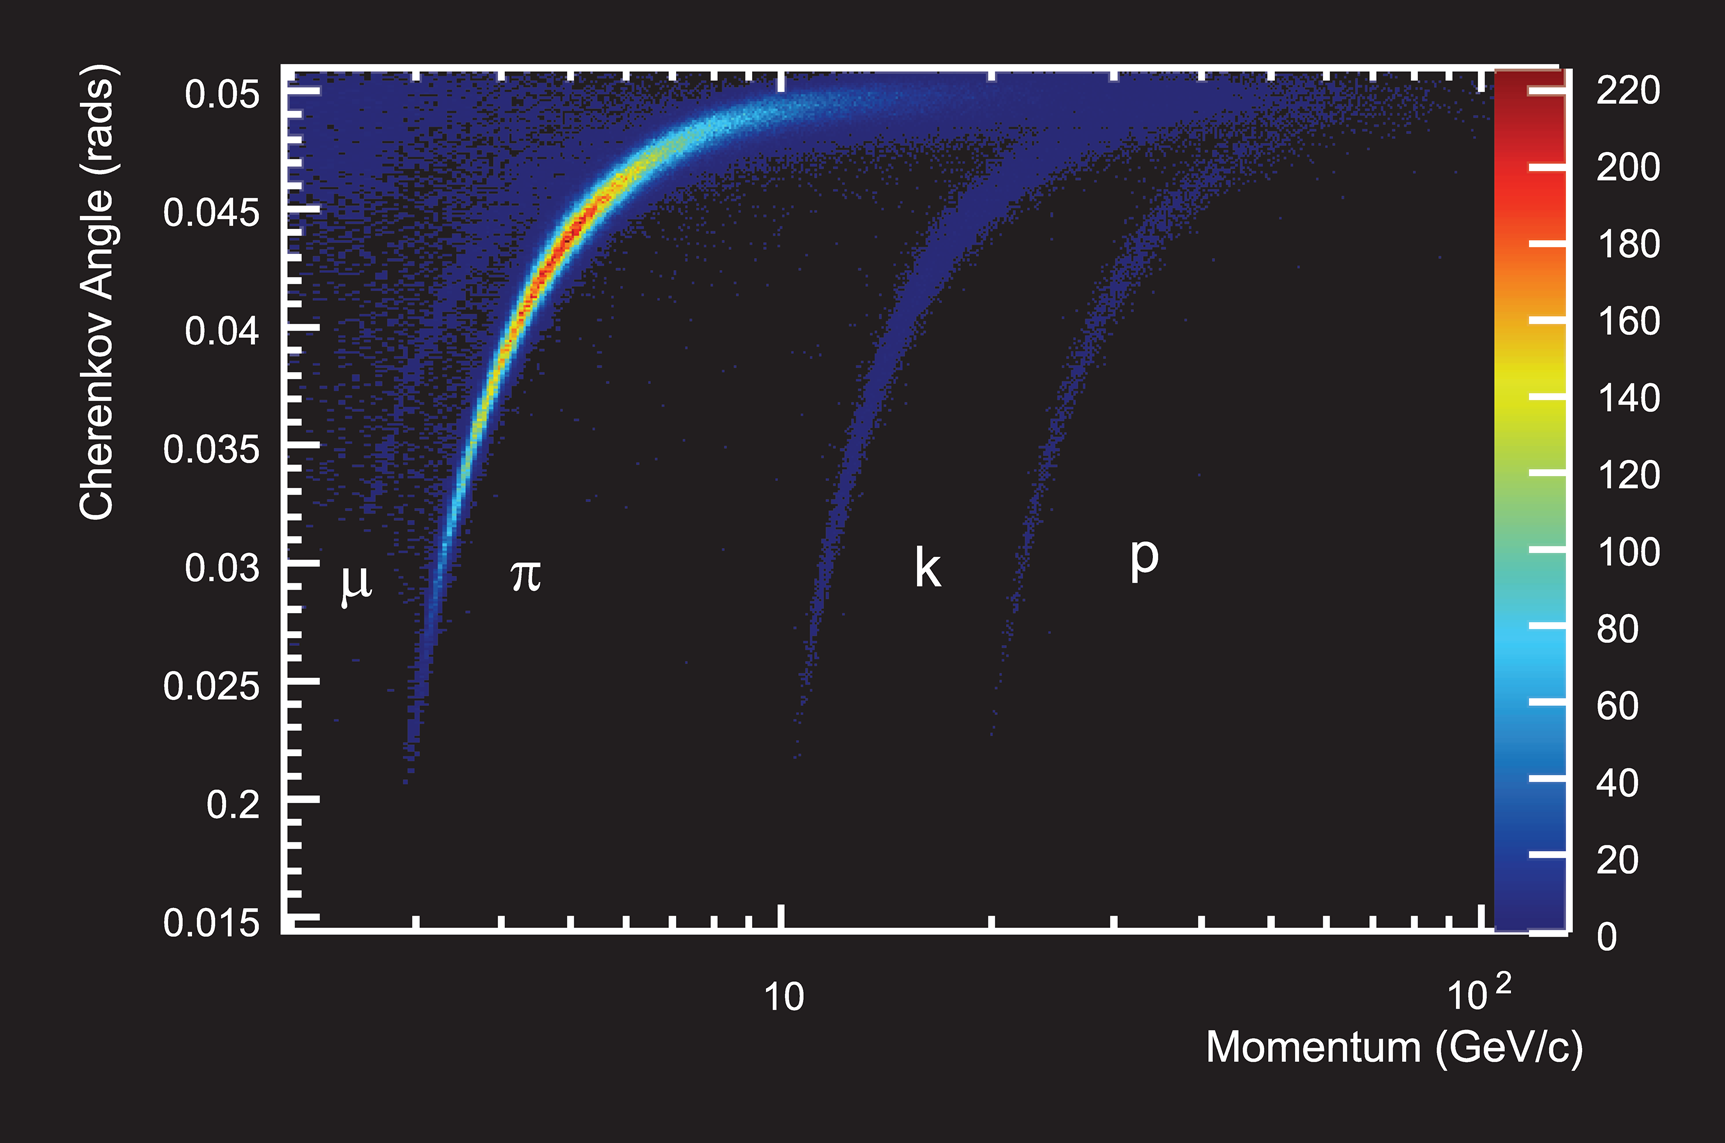
\includegraphics[width=0.59\linewidth]{images/RICH_ID.png}
        \caption{Possible particles and their momentum via a given Cherenkov angle.}
        \label{RICH}
    \end{figure}
%--------------%
    \item \textbf{Calorimeters}
    
    \textbf{Purpose:} Measuring the energy of electrons, photons, and hadrons via particle shower.
    
    \textbf{Features:}
    \begin{itemize}
        \item \textbf{Scintillating Pad Detector:} Electron/photon identification.
        \item \textbf{Preshower Detector:} Distinguishes electrons from hadrons.
        \item \textbf{Electromagnetic Calorimeter:} Measures energy of electrons and photons.
        \item \textbf{Hadronic Calorimeter:} Measures energy of hadrons (neutral hadrons like neutrons are primarily stopped here).
    \end{itemize}
%--------------%
    \item \textbf{Muon system}
    
    \textbf{Purpose:} Muon identification.
    
    \textbf{Features:} Five stations (M1–M5) using Multi-wire proportional chambers and gas-electron multipliers. The M1 station is before the calorimeters and M2 to M5 after, with shielding in between.
\end{enumerate}
